\chapter{Programação dinâmica}

\index{programação dinâmica}

\key{Programação dinâmica} é uma técnica que combina a corretude
da busca completa com a eficiência
dos algoritmos gulosos. A programação dinâmica pode ser aplicada se o
problema puder ser dividido em subproblemas sobrepostos
que podem ser resolvidos independentemente.

Existem dois usos para a programação dinâmica:

\begin{itemize}
\item
\key{Encontrar uma solução ótima}:
Queremos encontrar uma solução que seja
a maior possível ou a menor possível.
\item
\key{Contar o número de soluções}:
Queremos calcular o número total de
soluções possíveis.
\end{itemize}

Veremos primeiro como a programação dinâmica pode
ser usada para encontrar uma solução ótima,
e então usaremos a mesma ideia para
contar as soluções.

Entender a programação dinâmica é um marco
na carreira de todo programador competitivo.
Enquanto a ideia básica é simples,
o desafio é como aplicar
a programação dinâmica a diferentes problemas.
Este capítulo apresenta um conjunto de problemas clássicos
que são um bom ponto de partida.

\section{Problema das moedas}

Vamos primeiro nos concentrar em um problema que
já vimos no Capítulo 6:
Dado um conjunto de valores de moedas $\texttt{moedas} = \{c_1,c_2,\ldots,c_k\}$
e uma soma alvo de dinheiro $n$, nossa tarefa é
formar a soma $n$ usando o menor número possível de moedas.

No Capítulo 6, resolvemos o problema usando um
algoritmo guloso que sempre escolhe a maior
moeda possível.
O algoritmo guloso funciona, por exemplo,
quando as moedas são as moedas de euro,
mas no caso geral, o algoritmo guloso
não produz necessariamente uma solução ótima.

Agora é hora de resolver o problema de forma eficiente
usando programação dinâmica, para que o algoritmo
funcione para qualquer conjunto de moedas.
O algoritmo de programação dinâmica é baseado em uma função recursiva
que percorre todas as possibilidades de como
formar a soma, como um algoritmo de força bruta.
No entanto, o algoritmo de programação dinâmica
é eficiente porque
usa \emph{memoização} e
calcula a resposta para cada subproblema apenas uma vez.

\subsubsection{Formulação recursiva}

A ideia da programação dinâmica é
formular o problema recursivamente para
que a solução do problema possa ser
calculada a partir de soluções para subproblemas menores.
No problema das moedas, um problema recursivo natural
é o seguinte:
qual é o menor número de moedas
necessário para formar uma soma $x$?

Seja $\texttt{resolver}(x)$
o número mínimo
de moedas necessárias para uma soma $x$.
Os valores da função dependem dos
valores das moedas.
Por exemplo, se $\texttt{moedas} = \{1,3,4\}$,
os primeiros valores da função são os seguintes:

\[
\begin{array}{lcl}
\texttt{resolver}(0) & = & 0 \\
\texttt{resolver}(1) & = & 1 \\
\texttt{resolver}(2) & = & 2 \\
\texttt{resolver}(3) & = & 1 \\
\texttt{resolver}(4) & = & 1 \\
\texttt{resolver}(5) & = & 2 \\
\texttt{resolver}(6) & = & 2 \\
\texttt{resolver}(7) & = & 2 \\
\texttt{resolver}(8) & = & 2 \\
\texttt{resolver}(9) & = & 3 \\
\texttt{resolver}(10) & = & 3 \\
\end{array}
\]

Por exemplo, $\texttt{resolver}(10)=3$,
porque pelo menos 3 moedas são necessárias
para formar a soma 10.
A solução ótima é $3+3+4=10$.

A propriedade essencial de $\texttt{resolver}$ é
que seus valores podem ser
calculados recursivamente a partir de seus valores menores.
A ideia é focar na \emph{primeira}
moeda que escolhemos para a soma.
Por exemplo, no cenário acima,
a primeira moeda pode ser 1, 3 ou 4.
Se escolhermos primeiro a moeda 1,
a tarefa restante é formar a soma 9
usando o número mínimo de moedas,
que é um subproblema do problema original.
Claro, o mesmo se aplica às moedas 3 e 4.
Assim, podemos usar a seguinte fórmula recursiva
para calcular o número mínimo de moedas:
\begin{equation*}
\begin{split}
\texttt{resolver}(x) = \min( & \texttt{resolver}(x-1)+1, \\
                           & \texttt{resolver}(x-3)+1, \\
                           & \texttt{resolver}(x-4)+1).
\end{split}
\end{equation*}
O caso base da recursão é $\texttt{resolver}(0)=0$,
porque nenhuma moeda é necessária para formar uma soma vazia.
Por exemplo,
\[ \texttt{resolver}(10) = \texttt{resolver}(7)+1 = \texttt{resolver}(4)+2 = \texttt{resolver}(0)+3 = 3.\]

Agora estamos prontos para fornecer uma função recursiva geral
que calcula o número mínimo de
moedas necessárias para formar uma soma $x$:
\begin{equation*}
    \texttt{resolver}(x) = \begin{cases}
               \infty               & x < 0\\
               0               & x = 0\\
               \min_{c \in \texttt{moedas}} \texttt{resolver}(x-c)+1 & x > 0 \\
           \end{cases}
\end{equation*}

Primeiro, se $x<0$, o valor é $\infty$,
porque é impossível formar uma soma negativa
de dinheiro.
Então, se $x=0$, o valor é $0$,
porque nenhuma moeda é necessária para formar uma soma vazia.
Finalmente, se $x>0$, a variável $c$ percorre
todas as possibilidades de como escolher a primeira moeda
da soma.

Uma vez encontrada uma função recursiva que resolve o problema,
podemos implementar diretamente uma solução em C++
(a constante \texttt{INF} denota infinito):

\begin{lstlisting}
int resolver(int x) {
    if (x < 0) return INF;
    if (x == 0) return 0;
    int melhor = INF;
    for (auto c : moedas) {
        melhor = min(melhor, resolver(x-c)+1);
    }
    return melhor;
}
\end{lstlisting}

Ainda assim, esta função não é eficiente,
porque pode haver um número exponencial de maneiras
de construir a soma.
No entanto, a seguir veremos como tornar a
função eficiente usando uma técnica chamada memoização.

\subsubsection{Usando memoização}

\index{memoização}

A ideia da programação dinâmica é usar
\key{memoização} para calcular eficientemente
valores de uma função recursiva.
Isso significa que os valores da função
são armazenados em um array após o cálculo.
Para cada parâmetro, o valor da função
é calculado recursivamente apenas uma vez e, depois disso,
o valor pode ser recuperado diretamente do array.

Neste problema, usamos arrays
\begin{lstlisting}
bool pronto[N];
int valor[N];
\end{lstlisting}

onde $\texttt{pronto}[x]$ indica
se o valor de $\texttt{resolver}(x)$ foi calculado,
e se foi, $\texttt{valor}[x]$
contém esse valor.
A constante $N$ foi escolhida de forma
que todos os valores necessários caibam nos arrays.

Agora a função pode ser eficientemente
implementada da seguinte forma:

\begin{lstlisting}
int resolver(int x) {
    if (x < 0) return INF;
    if (x == 0) return 0;
    if (pronto[x]) return valor[x];
    int melhor = INF;
    for (auto c : moedas) {
        melhor = min(melhor, resolver(x-c)+1);
    }
    valor[x] = melhor;
    pronto[x] = true;
    return melhor;
}
\end{lstlisting}

A função lida com os casos base
$x<0$ e $x=0$ como anteriormente.
Então a função verifica em
$\texttt{pronto}[x]$ se
$\texttt{resolver}(x)$ já foi armazenado
em $\texttt{valor}[x]$,
e se foi, a função o retorna diretamente.
Caso contrário, a função calcula o valor
de $\texttt{resolver}(x)$
recursivamente e o armazena em $\texttt{valor}[x]$.

Esta função funciona de forma eficiente,
porque a resposta para cada parâmetro $x$
é calculada recursivamente apenas uma vez.
Depois que um valor de $\texttt{resolver}(x)$ é armazenado em $\texttt{valor}[x]$,
ele pode ser recuperado de forma eficiente sempre que a
função for chamada novamente com o parâmetro $x$.
A complexidade de tempo do algoritmo é $O(nk)$,
onde $n$ é a soma alvo e $k$ é o número de moedas.

Observe que também podemos construir o array \texttt{valor}
\emph{iterativamente} usando
um loop que simplesmente calcula todos os valores
de $\texttt{resolver}$ para os parâmetros $0 \ldots n$:
\begin{lstlisting}
valor[0] = 0;
for (int x = 1; x <= n; x++) {
    valor[x] = INF;
    for (auto c : moedas) {
        if (x-c >= 0) {
            valor[x] = min(valor[x], valor[x-c]+1);
        }
    }
}
\end{lstlisting}

Na verdade, a maioria dos programadores competitivos prefere esta
implementação, porque é mais curta e tem
menores fatores constantes.
De agora em diante, também usaremos implementações iterativas
em nossos exemplos.
Ainda assim, geralmente é mais fácil pensar em
soluções de programação dinâmica
em termos de funções recursivas.


\subsubsection{Construindo uma solução}

Às vezes, somos solicitados a encontrar o valor
de uma solução ótima e dar
um exemplo de como essa solução pode ser construída.
No problema das moedas, por exemplo,
podemos declarar outro array
que indica para
cada soma de dinheiro a primeira moeda
em uma solução ótima:
\begin{lstlisting}
int primeiro[N];
\end{lstlisting}
Então, podemos modificar o algoritmo da seguinte forma:
\begin{lstlisting}
valor[0] = 0;
for (int x = 1; x <= n; x++) {
    valor[x] = INF;
    for (auto c : moedas) {
        if (x-c >= 0 && valor[x-c]+1 < valor[x]) {
            valor[x] = valor[x-c]+1;
            primeiro[x] = c;
        }
    }
}
\end{lstlisting}
Depois disso, o seguinte código pode ser usado para
imprimir as moedas que aparecem em uma solução ótima para
a soma $n$:
\begin{lstlisting}
while (n > 0) {
    cout << primeiro[n] << "\n";
    n -= primeiro[n];
}
\end{lstlisting}

\subsubsection{Contando o número de soluções}

Vamos agora considerar outra versão
do problema das moedas, onde nossa tarefa é
calcular o número total de maneiras
de produzir uma soma $x$ usando as moedas.
Por exemplo, se $\texttt{moedas}=\{1,3,4\}$ e
$x=5$, existem um total de 6 maneiras:

\begin{multicols}{2}
\begin{itemize}
\item $1+1+1+1+1$
\item $1+1+3$
\item $1+3+1$
\item $3+1+1$
\item $1+4$
\item $4+1$
\end{itemize}
\end{multicols}

Novamente, podemos resolver o problema recursivamente.
Seja $\texttt{resolver}(x)$ o número de maneiras
de formarmos a soma $x$.
Por exemplo, se $\texttt{moedas}=\{1,3,4\}$,
então $\texttt{resolver}(5)=6$ e a fórmula recursiva é
\begin{equation*}
\begin{split}
\texttt{resolver}(x) = & \texttt{resolver}(x-1) + \\
                    & \texttt{resolver}(x-3) + \\
                    & \texttt{resolver}(x-4)  .
\end{split}
\end{equation*}

Então, a função recursiva geral é a seguinte:
\begin{equation*}
    \texttt{resolver}(x) = \begin{cases}
               0               & x < 0\\
               1               & x = 0\\
               \sum_{c \in \texttt{moedas}} \texttt{resolver}(x-c) & x > 0 \\
           \end{cases}
\end{equation*}

Se $x<0$, o valor é 0, porque não há soluções.
Se $x=0$, o valor é 1, porque só há uma maneira
de formar uma soma vazia.
Caso contrário, calculamos a soma de todos os valores
da forma $\texttt{resolver}(x-c)$ onde $c$ está em \texttt{moedas}.

O código a seguir constrói um array
$\texttt{contagem}$ tal que
$\texttt{contagem}[x]$ é igual
ao valor de $\texttt{resolver}(x)$
para $0 \le x \le n$:

\begin{lstlisting}
contagem[0] = 1;
for (int x = 1; x <= n; x++) {
    for (auto c : moedas) {
        if (x-c >= 0) {
            contagem[x] += contagem[x-c];
        }
    }
}
\end{lstlisting}

Muitas vezes, o número de soluções é tão grande
que não é necessário calcular o número exato,
mas é suficiente fornecer a resposta módulo $m$
onde, por exemplo, $m=10^9+7$.
Isso pode ser feito alterando o código para que
todos os cálculos sejam feitos módulo $m$.
No código acima, basta adicionar a linha
\begin{lstlisting}
        contagem[x] %= m;
\end{lstlisting}
após a linha
\begin{lstlisting}
        contagem[x] += contagem[x-c];
\end{lstlisting}

Agora discutimos todas as ideias básicas
da programação dinâmica.
Como a programação dinâmica pode ser usada
em muitas situações diferentes,
vamos agora passar por um conjunto de problemas
que mostram outros exemplos sobre as
possibilidades da programação dinâmica.

\section{Maior subsequência crescente}

\index{maior subsequência crescente}

Nosso primeiro problema é encontrar a
\key{maior subsequência crescente}
em um array de $n$ elementos.
Esta é uma sequência de comprimento máximo
de elementos do array
que vai da esquerda para a direita,
e cada elemento na sequência é maior
que o elemento anterior.
Por exemplo, no array

\begin{center}
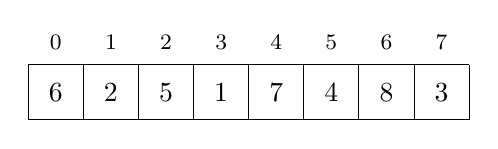
\begin{tikzpicture}[scale=0.7]
\draw (0,0) grid (8,1);
\node at (0.5,0.5) {$6$};
\node at (1.5,0.5) {$2$};
\node at (2.5,0.5) {$5$};
\node at (3.5,0.5) {$1$};
\node at (4.5,0.5) {$7$};
\node at (5.5,0.5) {$4$};
\node at (6.5,0.5) {$8$};
\node at (7.5,0.5) {$3$};

\footnotesize
\node at (0.5,1.4) {$0$};
\node at (1.5,1.4) {$1$};
\node at (2.5,1.4) {$2$};
\node at (3.5,1.4) {$3$};
\node at (4.5,1.4) {$4$};
\node at (5.5,1.4) {$5$};
\node at (6.5,1.4) {$6$};
\node at (7.5,1.4) {$7$};
\end{tikzpicture}
\end{center}
a maior subsequência crescente
contém 4 elementos:
\begin{center}
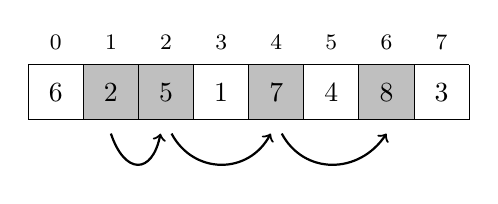
\begin{tikzpicture}[scale=0.7]
\fill[color=lightgray] (1,0) rectangle (2,1);
\fill[color=lightgray] (2,0) rectangle (3,1);
\fill[color=lightgray] (4,0) rectangle (5,1);
\fill[color=lightgray] (6,0) rectangle (7,1);
\draw (0,0) grid (8,1);
\node at (0.5,0.5) {$6$};
\node at (1.5,0.5) {$2$};
\node at (2.5,0.5) {$5$};
\node at (3.5,0.5) {$1$};
\node at (4.5,0.5) {$7$};
\node at (5.5,0.5) {$4$};
\node at (6.5,0.5) {$8$};
\node at (7.5,0.5) {$3$};

\draw[thick,->] (1.5,-0.25) .. controls (1.75,-1.00) and (2.25,-1.00) .. (2.4,-0.25);
\draw[thick,->] (2.6,-0.25) .. controls (3.0,-1.00) and (4.0,-1.00) .. (4.4,-0.25);
\draw[thick,->] (4.6,-0.25) .. controls (5.0,-1.00) and (6.0,-1.00) .. (6.5,-0.25);

\footnotesize
\node at (0.5,1.4) {$0$};
\node at (1.5,1.4) {$1$};
\node at (2.5,1.4) {$2$};
\node at (3.5,1.4) {$3$};
\node at (4.5,1.4) {$4$};
\node at (5.5,1.4) {$5$};
\node at (6.5,1.4) {$6$};
\node at (7.5,1.4) {$7$};
\end{tikzpicture}
\end{center}

Seja $\texttt{tamanho}(k)$ o comprimento da
maior subsequência crescente
que termina na posição $k$.
Assim, se calcularmos todos os valores de
$\texttt{tamanho}(k)$ onde $0 \le k \le n-1$,
descobriremos o comprimento da
maior subsequência crescente.
Por exemplo, os valores da função
para o array acima são os seguintes:
\[
\begin{array}{lcl}
\texttt{tamanho}(0) & = & 1 \\
\texttt{tamanho}(1) & = & 1 \\
\texttt{tamanho}(2) & = & 2 \\
\texttt{tamanho}(3) & = & 1 \\
\texttt{tamanho}(4) & = & 3 \\
\texttt{tamanho}(5) & = & 2 \\
\texttt{tamanho}(6) & = & 4 \\
\texttt{tamanho}(7) & = & 2 \\
\end{array}
\]

Por exemplo, $\texttt{tamanho}(6)=4$,
porque a maior subsequência crescente
que termina na posição 6 consiste em 4 elementos.

Para calcular um valor de $\texttt{tamanho}(k)$,
devemos encontrar uma posição $i<k$
para a qual $\texttt{array}[i]<\texttt{array}[k]$
e $\texttt{tamanho}(i)$ seja o maior possível.
Então sabemos que
$\texttt{tamanho}(k)=\texttt{tamanho}(i)+1$,
porque esta é uma maneira ótima de adicionar
$\texttt{array}[k]$ a uma subsequência.
No entanto, se não houver tal posição $i$,
então $\texttt{tamanho}(k)=1$,
o que significa que a subsequência contém apenas
$\texttt{array}[k]$.

Como todos os valores da função podem ser calculados
a partir de seus valores menores,
podemos usar programação dinâmica.
No código a seguir, os valores
da função serão armazenados em um array
$\texttt{tamanho}$.

\begin{lstlisting}
for (int k = 0; k < n; k++) {
    tamanho[k] = 1;
    for (int i = 0; i < k; i++) {
        if (array[i] < array[k]) {
            tamanho[k] = max(tamanho[k],tamanho[i]+1);
        }
    }
}
\end{lstlisting}

Este código funciona em tempo $O(n^2)$,
porque consiste em dois loops aninhados.
No entanto, também é possível implementar
o cálculo de programação dinâmica
de forma mais eficiente em tempo $O(n \log n)$.
Você consegue encontrar uma maneira de fazer isso?

\section{Caminhos em uma grade}

Nosso próximo problema é encontrar um caminho
do canto superior esquerdo para
o canto inferior direito
de uma grade $n \times n$, de forma que
só nos movamos para baixo e para a direita.
Cada quadrado contém um inteiro positivo,
e o caminho deve ser construído de forma
que a soma dos valores ao longo
do caminho seja a maior possível.

A figura a seguir mostra um caminho ideal
em uma grade:
\begin{center}
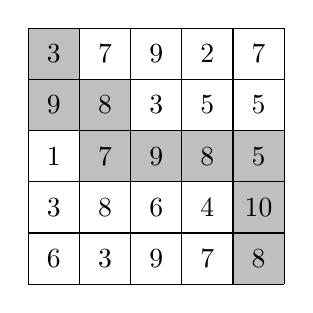
\begin{tikzpicture}[scale=.65]
  \begin{scope}
    \fill [color=lightgray] (0, 9) rectangle (1, 8);
    \fill [color=lightgray] (0, 8) rectangle (1, 7);
    \fill [color=lightgray] (1, 8) rectangle (2, 7);
    \fill [color=lightgray] (1, 7) rectangle (2, 6);
    \fill [color=lightgray] (2, 7) rectangle (3, 6);
    \fill [color=lightgray] (3, 7) rectangle (4, 6);
    \fill [color=lightgray] (4, 7) rectangle (5, 6);
    \fill [color=lightgray] (4, 6) rectangle (5, 5);
    \fill [color=lightgray] (4, 5) rectangle (5, 4);
    \draw (0, 4) grid (5, 9);
    \node at (0.5,8.5) {3};
    \node at (1.5,8.5) {7};
    \node at (2.5,8.5) {9};
    \node at (3.5,8.5) {2};
    \node at (4.5,8.5) {7};
    \node at (0.5,7.5) {9};
    \node at (1.5,7.5) {8};
    \node at (2.5,7.5) {3};
    \node at (3.5,7.5) {5};
    \node at (4.5,7.5) {5};
    \node at (0.5,6.5) {1};
    \node at (1.5,6.5) {7};
    \node at (2.5,6.5) {9};
    \node at (3.5,6.5) {8};
    \node at (4.5,6.5) {5};
    \node at (0.5,5.5) {3};
    \node at (1.5,5.5) {8};
    \node at (2.5,5.5) {6};
    \node at (3.5,5.5) {4};
    \node at (4.5,5.5) {10};
    \node at (0.5,4.5) {6};
    \node at (1.5,4.5) {3};
    \node at (2.5,4.5) {9};
    \node at (3.5,4.5) {7};
    \node at (4.5,4.5) {8};
  \end{scope}
\end{tikzpicture}
\end{center}
A soma dos valores no caminho é 67,
e esta é a maior soma possível em um caminho
do canto superior esquerdo para o canto inferior direito.

Assuma que as linhas e colunas da
grade são numeradas de 1 a $n$,
e $\texttt{valor}[y][x]$ é igual ao valor
do quadrado $(y,x)$.
Seja $\texttt{soma}(y,x)$ a soma máxima
em um caminho do canto superior esquerdo
para o quadrado $(y,x)$.
Agora $\texttt{soma}(n,n)$ nos diz
a soma máxima
do canto superior esquerdo para
o canto inferior direito.
Por exemplo, na grade acima,
$\texttt{soma}(5,5)=67$.

Podemos calcular recursivamente as somas
da seguinte forma:
\[ \texttt{soma}(y,x) = \max(\texttt{soma}(y,x-1),\texttt{soma}(y-1,x))+\texttt{valor}[y][x]\]


A fórmula recursiva é baseada na observação
de que um caminho que termina no quadrado $(y,x)$
pode vir do quadrado $(y,x-1)$
ou do quadrado $(y-1,x)$:
\begin{center}
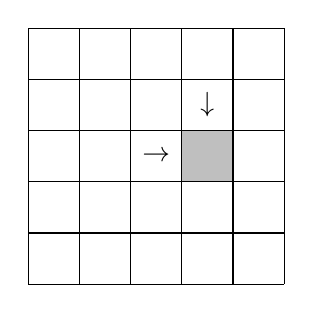
\begin{tikzpicture}[scale=.65]
  \begin{scope}
    \fill [color=lightgray] (3, 7) rectangle (4, 6);
    \draw (0, 4) grid (5, 9);
    
    \node at (2.5,6.5) {$\rightarrow$};
    \node at (3.5,7.5) {$\downarrow$};
    
  \end{scope}
\end{tikzpicture}
\end{center}

Assim, selecionamos a direção que maximiza
a soma.
Assumimos que $\texttt{soma}(y,x)=0$
se $y=0$ ou $x=0$ (porque tais caminhos não existem),
então a fórmula recursiva também funciona quando $y=1$ ou $x=1$.

Como a função \texttt{soma} possui dois parâmetros,
o array de programação dinâmica também possui duas dimensões.
Por exemplo, podemos usar um array
\begin{lstlisting}
int soma[N][N];
\end{lstlisting}
e calcular as somas da seguinte forma:
\begin{lstlisting}
for (int y = 1; y <= n; y++) {
    for (int x = 1; x <= n; x++) {
        soma[y][x] = max(soma[y][x-1],soma[y-1][x])+valor[y][x];
    }
}
\end{lstlisting}
A complexidade de tempo do algoritmo é $O(n^2)$.

\section{Problemas da mochila}

\index{mochila}

O termo \key{mochila} refere-se a problemas onde
um conjunto de objetos é dado, e
subconjuntos com algumas propriedades
precisam ser encontrados.
Os problemas da mochila podem ser resolvidos
usando programação dinâmica.

Nesta seção, vamos focar no seguinte
problema: Dada uma lista de pesos
$[w_1,w_2,\ldots,w_n]$,
determine todas as
somas que podem ser construídas usando os pesos.
Por exemplo, se os pesos forem
$[1,3,3,5]$, as seguintes somas são possíveis:

\begin{center}
\begin{tabular}{rrrrrrrrrrrrr}
 0 & 1 & 2 & 3 & 4 & 5 & 6 & 7 & 8 & 9 & 10 & 11 & 12 \\
\hline
 X & X & & X & X & X & X & X & X & X & & X & X \\
\end{tabular}
\end{center}

Neste caso, todas as somas entre $0 \ldots 12$
são possíveis, exceto 2 e 10.
Por exemplo, a soma 7 é possível porque nós
podemos selecionar os pesos $[1,3,3]$.

Para resolver o problema, vamos focar em subproblemas
onde usamos apenas os primeiros $k$ pesos
para construir somas.
Seja $\texttt{possivel}(x,k)=\textrm{verdadeiro}$ se
podemos construir uma soma $x$
usando os primeiros $k$ pesos,
e caso contrário $\texttt{possivel}(x,k)=\textrm{falso}$.
Os valores da função podem ser calculados recursivamente
da seguinte forma:
\[ \texttt{possivel}(x,k) = \texttt{possivel}(x-w_k,k-1) \lor \texttt{possivel}(x,k-1) \]
A fórmula é baseada no fato de que podemos
usar ou não o peso $w_k$ na soma.
Se usarmos $w_k$, a tarefa restante é
formar a soma $x-w_k$ usando os primeiros $k-1$ pesos,
e se não usarmos $w_k$,
a tarefa restante é formar a soma $x$
usando os primeiros $k-1$ pesos.
Como casos base,
\begin{equation*}
    \texttt{possivel}(x,0) = \begin{cases}
               \textrm{verdadeiro}    & x = 0\\
               \textrm{falso}   & x \neq 0 \\
           \end{cases}
\end{equation*}
porque se nenhum peso for usado,
só podemos formar a soma 0.

A tabela a seguir mostra todos os valores da função
para os pesos $[1,3,3,5]$ (o símbolo ''X''
indica os valores verdadeiros):

\begin{center}
\begin{tabular}{r|rrrrrrrrrrrrr}
$k \backslash x$ & 0 & 1 & 2 & 3 & 4 & 5 & 6 & 7 & 8 & 9 & 10 & 11 & 12 \\
\hline
 0 & X & \\
 1 & X & X \\
 2 & X & X & & X & X \\
 3 & X & X & & X & X & & X & X \\
 4 & X & X & & X & X & X & X & X & X & X & & X & X \\
\end{tabular}
\end{center}

Após calcular esses valores, $\texttt{possivel}(x,n)$
nos diz se podemos construir uma
soma $x$ usando \emph{todos} os pesos.

Seja $W$ a soma total dos pesos.
A seguinte solução de programação dinâmica em tempo $O(nW)$
corresponde à função recursiva:
\begin{lstlisting}
possivel[0][0] = true;
for (int k = 1; k <= n; k++) {
    for (int x = 0; x <= W; x++) {
        if (x-w[k] >= 0) possivel[x][k] |= possivel[x-w[k]][k-1];
        possivel[x][k] |= possivel[x][k-1];
    }
}
\end{lstlisting}

No entanto, aqui está uma implementação melhor que usa apenas
um array unidimensional $\texttt{possivel}[x]$
que indica se podemos construir um subconjunto com soma $x$.
O truque é atualizar o array da direita para a esquerda para
cada novo peso:
\begin{lstlisting}
possivel[0] = true;
for (int k = 1; k <= n; k++) {
    for (int x = W; x >= 0; x--) {
        if (possivel[x]) possivel[x+w[k]] = true;
    }
}
\end{lstlisting}

Observe que a ideia geral apresentada aqui pode ser usada
em muitos problemas de mochila.
Por exemplo, se recebermos objetos com pesos e valores,
podemos determinar para cada soma de peso o valor máximo
soma de um subconjunto.

\section{Distância de edição}

\index{distância de edição}
\index{distância de Levenshtein}

A \key{distância de edição} ou \key{distância de Levenshtein}\footnote{A distância
recebe o nome de V. I. Levenshtein, que a estudou em conexão com códigos binários \cite{lev66}.}
é o número mínimo de operações de edição
necessárias para transformar uma string
em outra.
As operações de edição permitidas são as seguintes:
\begin{itemize}
\item inserir um caractere (por exemplo, \texttt{ABC} $\rightarrow$ \texttt{ABCA})
\item remover um caractere (por exemplo, \texttt{ABC} $\rightarrow$ \texttt{AC})
\item modificar um caractere (por exemplo, \texttt{ABC} $\rightarrow$ \texttt{ADC})
\end{itemize}

Por exemplo, a distância de edição entre
\texttt{LOVE} e \texttt{MOVIE} é 2,
porque podemos primeiro realizar a operação
\texttt{LOVE} $\rightarrow$ \texttt{MOVE}
(modificar) e então a operação
\texttt{MOVE} $\rightarrow$ \texttt{MOVIE}
(inserir).
Este é o menor número possível de operações,
porque é claro que apenas uma operação não é suficiente.

Suponha que recebemos uma string \texttt{x}
de comprimento $n$ e uma string \texttt{y} de comprimento $m$,
e queremos calcular a distância de edição entre
\texttt{x} e \texttt{y}.
Para resolver o problema, definimos uma função
$\texttt{distancia}(a,b)$ que retorna a
distância de edição entre os prefixos
$\texttt{x}[0 \ldots a]$ e $\texttt{y}[0 \ldots b]$.
Assim, usando esta função, a distância de edição
entre \texttt{x} e \texttt{y} é igual a $\texttt{distancia}(n-1,m-1)$.

Podemos calcular os valores de \texttt{distancia}
da seguinte forma:
\begin{equation*}
\begin{split}
\texttt{distancia}(a,b) = \min(& \texttt{distancia}(a,b-1)+1, \\
                           & \texttt{distancia}(a-1,b)+1, \\
                           & \texttt{distancia}(a-1,b-1)+\texttt{custo}(a,b)).
\end{split}
\end{equation*}
Aqui $\texttt{custo}(a,b)=0$ se $\texttt{x}[a]=\texttt{y}[b]$,
e caso contrário $\texttt{custo}(a,b)=1$.
A fórmula considera as seguintes maneiras de
editar a string \texttt{x}:
\begin{itemize}
\item $\texttt{distancia}(a,b-1)$: inserir um caractere no final de \texttt{x}
\item $\texttt{distancia}(a-1,b)$: remover o último caractere de \texttt{x}
\item $\texttt{distancia}(a-1,b-1)$: combinar ou modificar o último caractere de \texttt{x}
\end{itemize}
Nos dois primeiros casos, uma operação de edição é necessária
(inserir ou remover).
No último caso, se $\texttt{x}[a]=\texttt{y}[b]$,
podemos combinar os últimos caracteres sem editar,
e caso contrário, uma operação de edição é necessária (modificar).

A tabela a seguir mostra os valores de \texttt{distancia}
no caso de exemplo:
\begin{center}
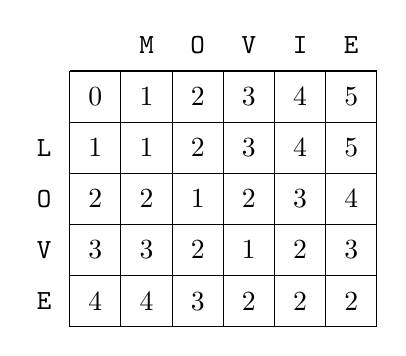
\begin{tikzpicture}[scale=.65]
  \begin{scope}
    %\fill [color=lightgray] (5, -3) rectangle (6, -4);
    \draw (1, -1) grid (7, -6);
    
    \node at (0.5,-2.5) {\texttt{L}};
    \node at (0.5,-3.5) {\texttt{O}};
    \node at (0.5,-4.5) {\texttt{V}};
    \node at (0.5,-5.5) {\texttt{E}};

    \node at (2.5,-0.5) {\texttt{M}};
    \node at (3.5,-0.5) {\texttt{O}};
    \node at (4.5,-0.5) {\texttt{V}};
    \node at (5.5,-0.5) {\texttt{I}};
    \node at (6.5,-0.5) {\texttt{E}};

    \node at (1.5,-1.5) {$0$};
    \node at (1.5,-2.5) {$1$};
    \node at (1.5,-3.5) {$2$};
    \node at (1.5,-4.5) {$3$};
    \node at (1.5,-5.5) {$4$};
    \node at (2.5,-1.5) {$1$};
    \node at (2.5,-2.5) {$1$};
    \node at (2.5,-3.5) {$2$};
    \node at (2.5,-4.5) {$3$};
    \node at (2.5,-5.5) {$4$};
    \node at (3.5,-1.5) {$2$};
    \node at (3.5,-2.5) {$2$};
    \node at (3.5,-3.5) {$1$};
    \node at (3.5,-4.5) {$2$};
    \node at (3.5,-5.5) {$3$};
    \node at (4.5,-1.5) {$3$};
    \node at (4.5,-2.5) {$3$};
    \node at (4.5,-3.5) {$2$};
    \node at (4.5,-4.5) {$1$};
    \node at (4.5,-5.5) {$2$};
    \node at (5.5,-1.5) {$4$};
    \node at (5.5,-2.5) {$4$};
    \node at (5.5,-3.5) {$3$};
    \node at (5.5,-4.5) {$2$};
    \node at (5.5,-5.5) {$2$};
    \node at (6.5,-1.5) {$5$};
    \node at (6.5,-2.5) {$5$};
    \node at (6.5,-3.5) {$4$};
    \node at (6.5,-4.5) {$3$};
    \node at (6.5,-5.5) {$2$};
  \end{scope}
\end{tikzpicture}
\end{center}

O canto inferior direito da tabela
nos diz que a distância de edição entre
\texttt{LOVE} e \texttt{MOVIE} é 2.
A tabela também mostra como construir
a menor sequência de operações de edição.
Neste caso, o caminho é o seguinte:

\begin{center}
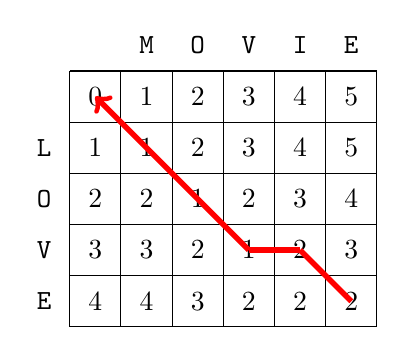
\begin{tikzpicture}[scale=.65]
  \begin{scope}
    \draw (1, -1) grid (7, -6);
    
    \node at (0.5,-2.5) {\texttt{L}};
    \node at (0.5,-3.5) {\texttt{O}};
    \node at (0.5,-4.5) {\texttt{V}};
    \node at (0.5,-5.5) {\texttt{E}};

    \node at (2.5,-0.5) {\texttt{M}};
    \node at (3.5,-0.5) {\texttt{O}};
    \node at (4.5,-0.5) {\texttt{V}};
    \node at (5.5,-0.5) {\texttt{I}};
    \node at (6.5,-0.5) {\texttt{E}};

    \node at (1.5,-1.5) {$0$};
    \node at (1.5,-2.5) {$1$};
    \node at (1.5,-3.5) {$2$};
    \node at (1.5,-4.5) {$3$};
    \node at (1.5,-5.5) {$4$};
    \node at (2.5,-1.5) {$1$};
    \node at (2.5,-2.5) {$1$};
    \node at (2.5,-3.5) {$2$};
    \node at (2.5,-4.5) {$3$};
    \node at (2.5,-5.5) {$4$};
    \node at (3.5,-1.5) {$2$};
    \node at (3.5,-2.5) {$2$};
    \node at (3.5,-3.5) {$1$};
    \node at (3.5,-4.5) {$2$};
    \node at (3.5,-5.5) {$3$};
    \node at (4.5,-1.5) {$3$};
    \node at (4.5,-2.5) {$3$};
    \node at (4.5,-3.5) {$2$};
    \node at (4.5,-4.5) {$1$};
    \node at (4.5,-5.5) {$2$};
    \node at (5.5,-1.5) {$4$};
    \node at (5.5,-2.5) {$4$};
    \node at (5.5,-3.5) {$3$};
    \node at (5.5,-4.5) {$2$};
    \node at (5.5,-5.5) {$2$};
    \node at (6.5,-1.5) {$5$};
    \node at (6.5,-2.5) {$5$};
    \node at (6.5,-3.5) {$4$};
    \node at (6.5,-4.5) {$3$};
    \node at (6.5,-5.5) {$2$};

    \path[draw=red,thick,-,line width=2pt] (6.5,-5.5) -- (5.5,-4.5);
    \path[draw=red,thick,-,line width=2pt] (5.5,-4.5) -- (4.5,-4.5);
    \path[draw=red,thick,->,line width=2pt] (4.5,-4.5) -- (1.5,-1.5);
  \end{scope}
\end{tikzpicture}
\end{center}

Os últimos caracteres de \texttt{LOVE} e \texttt{MOVIE}
são iguais, então a distância de edição entre eles
é igual à distância de edição entre \texttt{LOV} e \texttt{MOVI}.
Podemos usar uma operação de edição para remover o
caractere \texttt{I} de \texttt{MOVI}.
Assim, a distância de edição é um a mais que
a distância de edição entre \texttt{LOV} e \texttt{MOV}, etc.

\section{Contando os ladrilhos}

Às vezes, os estados de uma solução de programação dinâmica
são mais complexos do que combinações fixas de números.
Como exemplo,
considere o problema de calcular
o número de maneiras distintas de
preencher uma grade $n \times m$ usando
ladrilhos de tamanho $1 \times 2$ e $2 \times 1$.
Por exemplo, uma solução válida
para a grade $4 \times 7$ é
\begin{center}
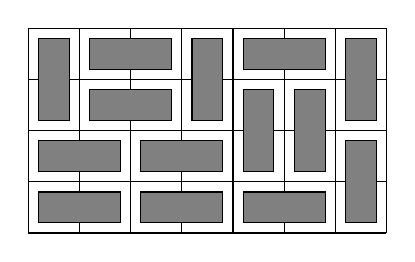
\begin{tikzpicture}[scale=.65]
    \draw (0,0) grid (7,4);
    \draw[fill=gray] (0+0.2,0+0.2) rectangle (2-0.2,1-0.2);
    \draw[fill=gray] (2+0.2,0+0.2) rectangle (4-0.2,1-0.2);
    \draw[fill=gray] (4+0.2,0+0.2) rectangle (6-0.2,1-0.2);
    \draw[fill=gray] (0+0.2,1+0.2) rectangle (2-0.2,2-0.2);
    \draw[fill=gray] (2+0.2,1+0.2) rectangle (4-0.2,2-0.2);
    \draw[fill=gray] (1+0.2,2+0.2) rectangle (3-0.2,3-0.2);
    \draw[fill=gray] (1+0.2,3+0.2) rectangle (3-0.2,4-0.2);
    \draw[fill=gray] (4+0.2,3+0.2) rectangle (6-0.2,4-0.2);

    \draw[fill=gray] (0+0.2,2+0.2) rectangle (1-0.2,4-0.2);
    \draw[fill=gray] (3+0.2,2+0.2) rectangle (4-0.2,4-0.2);
    \draw[fill=gray] (6+0.2,2+0.2) rectangle (7-0.2,4-0.2);
    \draw[fill=gray] (4+0.2,1+0.2) rectangle (5-0.2,3-0.2);
    \draw[fill=gray] (5+0.2,1+0.2) rectangle (6-0.2,3-0.2);
    \draw[fill=gray] (6+0.2,0+0.2) rectangle (7-0.2,2-0.2);

\end{tikzpicture}
\end{center}
e o número total de soluções é 781.

O problema pode ser resolvido usando programação dinâmica
percorrendo a grade linha por linha.
Cada linha em uma solução pode ser representada como uma
string que contém $m$ caracteres do conjunto
$\{\sqcap, \sqcup, \sqsubset, \sqsupset \}$.
Por exemplo, a solução acima consiste em quatro linhas
que correspondem às seguintes strings:
\begin{itemize}
\item
$\sqcap \sqsubset \sqsupset \sqcap \sqsubset \sqsupset \sqcap$
\item
$\sqcup \sqsubset \sqsupset \sqcup \sqcap \sqcap \sqcup$
\item
$\sqsubset \sqsupset \sqsubset \sqsupset \sqcup \sqcup \sqcap$ 
\item
$\sqsubset \sqsupset \sqsubset \sqsupset \sqsubset \sqsupset \sqcup$
\end{itemize}

Seja $\texttt{contar}(k,x)$ o número de maneiras de
construir uma solução para as linhas $1 \ldots k$
da grade, de modo que a string $x$ corresponda à linha $k$.
É possível usar a programação dinâmica aqui,
porque o estado de uma linha é restringido
apenas pelo estado da linha anterior.

Uma solução é válida se a linha $1$ não contiver
o caractere $\sqcup$,
a linha $n$ não contiver o caractere $\sqcap$,
e todas as linhas consecutivas forem \emph{compatíveis}.
Por exemplo, as linhas
$\sqcup \sqsubset \sqsupset \sqcup \sqcap \sqcap \sqcup$ e
$\sqsubset \sqsupset \sqsubset \sqsupset \sqcup \sqcup \sqcap$ 
são compatíveis, enquanto as linhas
$\sqcap \sqsubset \sqsupset \sqcap \sqsubset \sqsupset \sqcap$ e
$\sqsubset \sqsupset \sqsubset \sqsupset \sqsubset \sqsupset \sqcup$
não são compatíveis.

Como uma linha consiste em $m$ caracteres e existem
quatro opções para cada caractere, o número de linhas distintas
é no máximo $4^m$.
Assim, a complexidade de tempo da solução é
$O(n 4^{2m})$ porque podemos percorrer os
$O(4^m)$ estados possíveis para cada linha,
e para cada estado, existem $O(4^m)$
estados possíveis para a linha anterior.
Na prática, é uma boa ideia girar a grade
para que o lado mais curto tenha comprimento $m$,
porque o fator $4^{2m}$ domina a complexidade de tempo.

É possível tornar a solução mais eficiente
usando uma representação mais compacta para as linhas.
Acontece que é suficiente saber quais
colunas da linha anterior contêm o quadrado superior
de um ladrilho vertical.
Assim, podemos representar uma linha usando apenas caracteres
$\sqcap$ e $\Box$, onde $\Box$ é uma combinação
de caracteres
$\sqcup$, $\sqsubset$ e $\sqsupset$.
Usando esta representação, existem apenas
$2^m$ linhas distintas e a complexidade de tempo é
$O(n 2^{2m})$.

Como nota final, há também uma fórmula direta surpreendente
para calcular o número de ladrilhos\footnote{Surpreendentemente,
esta fórmula foi descoberta em 1961 por duas equipes de pesquisa \cite{kas61,tem61}
que trabalharam de forma independente.}:
\[ \prod_{a=1}^{\lceil n/2 \rceil} \prod_{b=1}^{\lceil m/2 \rceil} 4 \cdot (\cos^2 \frac{\pi a}{n + 1} + \cos^2 \frac{\pi b}{m+1})\]
Esta fórmula é muito eficiente, pois calcula
o número de ladrilhos em tempo $O(nm)$,
mas como a resposta é um produto de números reais,
um problema ao usar a fórmula é
como armazenar os resultados intermediários com precisão.
